
%\subsubsection{ESMF\_RegridDistrb}
%
%{\sf DESCRIPTION:\\}
%Regrid options for Field data motion supported by ESMF.
%
%Valid values are:
%\begin{description}
%   \item [ESMF\_REGRIDDISTRB\_BOTH]
%         Redistribute both source and destination Fields.
%   \item [ESMF\_REGRIDDISTRB\_DEST]
%         Redistribute destination Field.
%   \item [ESMF\_REGRIDDISTRB\_NONE]
%         No data motion required or undefined.
%   \item [ESMF\_REGRIDDISTRB\_SOURCE]
%         Redistribute source Field.
%\end{description}


\subsubsection{ESMF\_RegridMethod}

{\sf DESCRIPTION:\\}
General Regrid methods supported by ESMF.

Valid values are:
\begin{description}
%  \item [ESMF\_REGRID\_METHOD\_ADJOINT]
%        Create adjoint of existing regrid
\item[ESMF\_REGRID\_METHOD\_BICUBIC ] not implemented yet

     Like the bilinear remapping, bicubic remapping is applicable
     only for logically-rectangular or block-structured logically-rectangular
     grids.  The bicubic remapping exactly follows the bilinear remapping except
     that four weights for each corner point are required.  Thus, num\_wts
     is set to four for this option.  The bicubic remapping is

\begin{eqnarray}\label{eq:bicubic}
f_P & = & 
    (1 - \beta^2(3-2\beta))(1 - \alpha^2(3-2\alpha))f(i  ,j  ) + \nonumber \\
& & (1 - \beta^2(3-2\beta))     \alpha^2(3-2\alpha) f(i+1,j  ) + \nonumber \\
& &      \beta^2(3-2\beta)      \alpha^2(3-2\alpha) f(i+1,j+1) + \nonumber \\
& &      \beta^2(3-2\beta) (1 - \alpha^2(3-2\alpha))f(i  ,j+1) + \nonumber \\
& & (1 - \beta^2(3-2\beta))\alpha  (\alpha-1)^2 
                        {{\partial f}\over{\partial i}}(i  ,j  ) + \nonumber \\
& & (1 - \beta^2(3-2\beta))\alpha^2(\alpha-1) 
                        {{\partial f}\over{\partial i}}(i+1,j  ) + \nonumber \\
& &      \beta^2(3-2\beta) \alpha^2(\alpha-1)
                        {{\partial f}\over{\partial i}}(i+1,j+1) + \nonumber \\
& &      \beta^2(3-2\beta) \alpha  (\alpha-1)^2 
                        {{\partial f}\over{\partial i}}(i  ,j+1) + \nonumber \\
& & \beta  (\beta-1)^2(1 - \alpha^2(3-2\alpha))
                        {{\partial f}\over{\partial j}}(i  ,j  ) + \nonumber \\
& & \beta  (\beta-1)^2     \alpha^2(3-2\alpha) 
                        {{\partial f}\over{\partial j}}(i+1,j  ) + \nonumber \\
& & \beta^2(\beta-1)       \alpha^2(3-2\alpha)
                        {{\partial f}\over{\partial j}}(i+1,j+1) + \nonumber \\
& & \beta^2(\beta-1)  (1 - \alpha^2(3-2\alpha)) 
                        {{\partial f}\over{\partial j}}(i  ,j+1) + \nonumber \\
& & \alpha  (\alpha-1)^2\beta  (\beta-1)^2
           {{\partial^2 f}\over{\partial i \partial j}}(i  ,j  ) + \nonumber \\
& & \alpha^2(\alpha-1)  \beta  (\beta-1)^2 
           {{\partial^2 f}\over{\partial i \partial j}}(i+1,j  ) + \nonumber \\
& & \alpha^2(\alpha-1)  \beta^2(\beta-1)
           {{\partial^2 f}\over{\partial i \partial j}}(i+1,j+1) + \nonumber \\
& & \alpha  (\alpha-1)^2\beta^2(\beta-1)
           {{\partial^2 f}\over{\partial i \partial j}}(i  ,j+1)
\end{eqnarray}

     where $\alpha$ and $\beta$ are identical to those found in the bilinear
     case and are found using an identical algorithm.  Note that unlike the
     conservative remappings, the gradients here are gradients with respect to
     the {\em logical} variable and not latitude or longitude.  Lastly, the four
     weights corresponding to each address pair correspond to the weight
     multiplying the field value at the point, the weight multiplying the
     gradient with respect to $i$, the weight multiplying the gradient with
     respect to $j$, and the weight multiplying the cross gradient in that order.

\item [ESMF\_REGRID\_METHOD\_BILINEAR]
     The bilinear regridding methods uses a local bilinear approximation
     to interpolate to a point in a quadrilateral grid.  This is applicable
     only for logically-rectangular or block-structured logically-rectangular
     grids.  Standard bilinear interpolation schemes can be found in many textbooks.
     Here we present a more general scheme which uses a local bilinear approximation
     to interpolate to a point in a quadrilateral grid.  Consider the grid points
     shown in Fig.~\ref{fig:quad} labelled with logically-rectangular indices
     (e.g. $(i,j)$).

\begin{figure}
\caption{A general quadrilateral grid. \label{fig:quad}}
\begin{picture}(10,10)

\put(1.0,1.0){\line(2,1){5.0}}
\put(6.0,3.5){\line(1,2){2.5}}
\put(1.0,1.0){\line(1,2){2.5}}
\put(3.5,6.0){\line(2,1){5.0}}

\put(1.0,1.0){\circle*{0.1}}
\put(6.0,3.5){\circle*{0.1}}
\put(3.5,6.0){\circle*{0.1}}
\put(8.5,8.5){\circle*{0.1}}
\put(5.25,5.0){\circle*{0.1}}

\put(0.75,0.5 ){1 $(i,j)$}
\put(6.25,3.25){2 $(i+1,j)$}
\put(1.75,6.0 ){$(i,j+1)$ 4}
\put(8.75,8.5 ){3 $(i+1,j+1)$}
\put(5.0 ,5.0 ){$P$}

\end{picture}
\end{figure}

     Let the latitude-longitude coordinates of point 1 be $(\theta(i,j),\phi(i,j))$,
     the coordinates of point 2 be $(\theta(i+1,j),\phi(i+1,j))$, etc. 
     Now let $\alpha$ and $\beta$ be
     continuous local coordinates such that the coordinates $(\alpha,\beta)$
     of point 1 are $(0,0)$, point 2 are $(1,0)$, point 3 are $(1,1)$ and
     point 4 are $(0,1)$.  If point $P$ lies inside the cell formed by the four
     points above, the function $f$ at point $P$ can be approximated by
\begin{eqnarray}\label{eq:bilinear}
f_P & = & (1-\alpha)(1-\beta)f(i,j) + \alpha(1-\beta)f(i+1,j) + \nonumber \\
    &   & \alpha\beta f(i+1,j+1) + (1-\alpha)\beta f(i,j+1)  \\
    & = & w_1 f(i,j) + w_2 f(i+1,j) + w_3 f(i+1,j+1) + w_4 f(i,j+1). \nonumber
\end{eqnarray}

     The remapping weights must therefore be computed by finding $\alpha$ and
     $\beta$ at point $P$.  

     The latitude-longitude coordinates $(\theta,\phi)$ of point $P$ are known
     and can also be approximated by
\begin{eqnarray}\label{eq:thetaphi}
\theta & = & (1-\alpha)(1-\beta)\theta_1 + \alpha(1-\beta)\theta_2 + \nonumber
          \alpha\beta \theta_3 + (1-\alpha)\beta \theta_4 \\
\phi   & = & (1-\alpha)(1-\beta)\phi_1   + \alpha(1-\beta)\phi_2 +
          \alpha\beta \phi_3 + (1-\alpha)\beta \phi_4.
\end{eqnarray}

     Because (\ref{eq:thetaphi}) is nonlinear in $\alpha$ and $\beta$, we must
     linearize and iterate toward a solution.  Differentiating 
     (\ref{eq:thetaphi}) results in
\begin{equation}
\left[\begin{array}{c} \delta\theta \\ \delta\phi \end{array}\right] = A
\left[\begin{array}{c} \delta\alpha \\ \delta\beta \end{array}\right],
\end{equation}

     where

\begin{equation}
A = \left[\begin{array}{cc}
(\theta_2-\theta_1) + (\theta_1-\theta_4+\theta_3-\theta_2)\beta &
(\theta_4-\theta_1) + (\theta_1-\theta_4+\theta_3-\theta_2)\alpha \\
(\phi_2-\phi_1) + (\phi_1-\phi_4+\phi_3-\phi_2)\beta &
(\phi_4-\phi_1) + (\phi_1-\phi_4+\phi_3-\phi_2)\alpha
\end{array}\right].
\end{equation}

     Inverting this system,

\begin{equation}\label{eq:dalpha}
\delta\alpha = \left|\begin{array}{cc}
\delta\theta &
(\theta_4-\theta_1) + (\theta_1-\theta_4+\theta_3-\theta_2)\alpha \\
\delta\phi &
(\phi_4-\phi_1) + (\phi_1-\phi_4+\phi_3-\phi_2)\alpha 
\end{array}\right| \div \det(A),
\end{equation}

     and

\begin{equation}\label{eq:dbeta}
\delta\beta = \left|\begin{array}{cc}
(\theta_2-\theta_1) + (\theta_1-\theta_4+\theta_3-\theta_2)\beta &
\delta\theta \\
(\phi_2-\phi_1) + (\phi_1-\phi_4+\phi_3-\phi_2)\beta &
\delta\phi 
\end{array}\right| \div \det(A).
\end{equation}

     Starting with an initial guess for $\alpha$ and $\beta$ (say 
     $\alpha=\beta=0$), equations~(\ref{eq:dalpha}) and (\ref{eq:dbeta})
     can be iterated until $\delta\alpha$ and $\delta\beta$ are suitably small.
     The weights can then be computed from (\ref{eq:bilinear}).  Note that
     for simple latitude-longitude grids, this iteration will converge in the
     first iteration.

     In order to compute the weights using this general bilinear iteration,
     it must be determined in which box the point $P$ resides.  Because this
     method is valid only for logically-rectangular grids, the sweep algorithm
     can be optimized to take advantage of this restriction.  The sweep
     method currently in ESMF steps through each data point $P$ on the destination
     grid.  For each destination point, it then loops through the cells on the
     source grid, comparing the coordinates of point $P$ with the bounding box
     formed by each cell's minimum and maximum coordinates.  Most source cells can
     be efficiently eliminated from the sweep via this simple test.  This loop is
     further optimized by tracking the index of the source cell containing the
     previous point and using that as the initial starting index for the next
     point's sweep, since both grids are logically ordered.  Please see
     Figure \ref{fig:BilinearSweep} for an illustration of the sweep algorithm.

\begin{center}
\begin{figure}
\caption{Illustration of the Bilinear Sweep Algorithm. }
\label{fig:BilinearSweep}
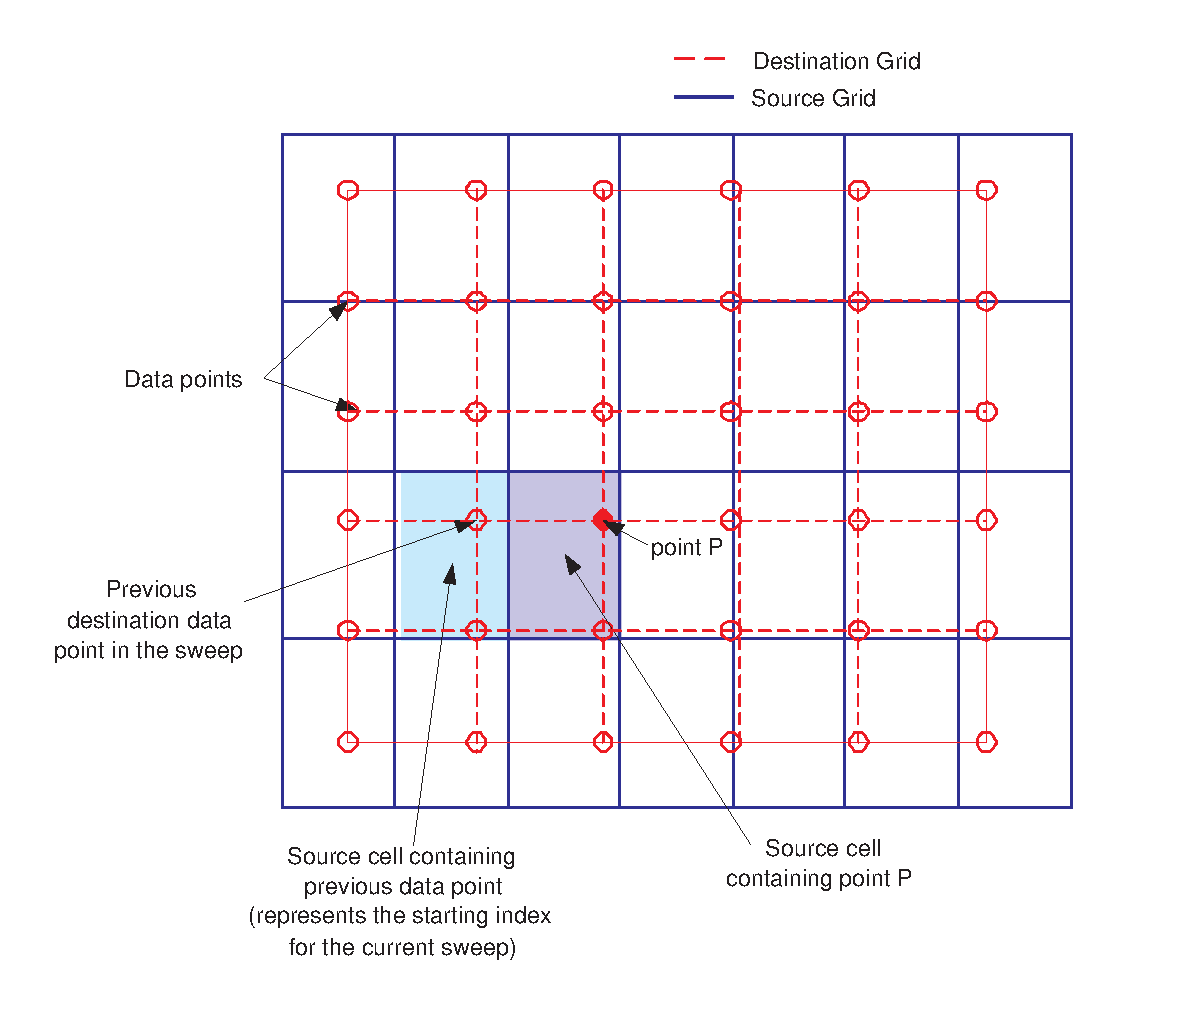
\includegraphics{BilinearSweep2002}
\end{figure}
\end{center}



%\item[ESMF\_REGRID\_METHOD\_CONSERV1 and ESMF\_REGRID\_METHOD\_CONSERV2]
\item[ESMF\_REGRID\_METHOD\_CONSERV1]
     First-order and second-order conservative remapping share a common
     algorithm, though currently only first-order has been implemented.
     ESMF implements a conservative remapping scheme described in detail
     elsewhere \cite{Jones1999}.  A brief outline will be given
     here to aid the user in understanding this regridding algorithm.

     To compute a flux on a new (destination) grid which results in the same
     energy or water exchange as a flux $f$ on an old (source) grid, the
     destination flux $F$ at a destination grid cell $k$ must satisfy

\begin{equation}\label{eq:local}
\overline{F}_k = {1\over{A_k}}\int\int_{A_k} fdA,
\end{equation}

     where $\overline{F}$ is the area-averaged flux and $A_k$ is the area of
     cell $k$. Because the integral in (\ref{eq:local}) is over the area of 
     the destination grid cell, only those cells on the source grid that are
     covered at least partly by the destination grid cell contribute to the
     value of the flux on the destination grid.  If cell $k$ overlaps $N$ cells
     on the source grid, the remapping can be written as 

\begin{equation}\label{eq:rmpsum}
\overline{F}_k = 
{1\over{A_k}} \sum_{n=1}^N \int\int_{A_{nk}} f_ndA,
\end{equation}

     where $A_{nk}$ is the area of the source grid cell $n$ covered by the
     destination grid cell $k$, and $f_n$ is the local value of the flux in the
     source grid cell (see Figure~\ref{fig:grids}).  Note that (\ref{eq:rmpsum})
     is normalized by the destination area $A_k$ corresponding to the
     {\tt ESMF\_RegridNormOpt} value of {\tt ESMF\_REGRID\_NORM\_DSTAREA}.  The
     sum of the weights for a destination cell $k$ in this case would be between
     0 and 1 and would be the area fraction if $f_n$ were identically 1 
     everywhere on the source grid.  The normalization option
     {\tt ESMF\_REGRID\_NORM\_FRACAREA} would actually divide by the area of the
     source grid overlapped by cell $k$: 

\begin{equation}
\sum_{n=1}^N \int\int_{A_{nk}}dA.
\end{equation}

     For this normalization option, remapping a function $f$ which is 1
     everywhere on the source grid would result in a function $F$ that is
     exactly one wherever the destination grid overlaps a non-masked source
     grid cell and zero otherwise.  A normalization option of
     {\tt ESMF\_REGRID\_NORM\_NONE} would result in the actual angular area
     participating in the remapping.

     Assuming $f_n$ is constant across a source grid cell, (\ref{eq:rmpsum})
     would lead to the first-order area-weighted schemes used in current coupled
     models.  A more accurate form of the remapping is obtained by using 

\begin{equation}\label{eq:gradient}
f_n = \overline{f}_n + 
                   \nabla_n f\cdot({\vec{r}} - \vec{r}_n),
\end{equation}

     where $\nabla_n f$ is the gradient of the flux in cell $n$ and $\vec{r}_n$
     is the centroid of cell $n$ defined by

 \begin{equation}\label{eq:centroid}
\vec{r}_n = {1\over{A_n}}\int\int_{A_n}\vec{r}dA.
\end{equation}

     Such a distribution satisfies the conservation constraint and is equivalent
     to the first terms of a Taylor series expansion of $f$ around $\vec{r}_n$.
     The remapping is thus second-order accurate if $\nabla_n f$ is at least a 
     first-order approximation to the gradient.

     The remapping can now be expanded in spherical coordinates as 

\begin{equation}\label{eq:remap}
\overline{F}_k = \sum_{n=1}^{N} \left[\overline{f}_n w_{1nk} + 
\left({{\partial f}\over{\partial \theta}}\right)_n w_{2nk} +
\left({1\over{\cos\theta}}{{\partial f}\over{\partial \phi}}\right)_n w_{3nk}
\right],
\end{equation}

     where $\theta$ is latitude, $\phi$ is longitude and the three remapping
     weights are

\begin{equation}\label{eq:weights1}
w_{1nk} = {1\over{A_k}}\int\int_{A_{nk}}dA, \\
\end{equation}
\begin{eqnarray}\label{eq:weights2}
w_{2nk} & = & {1\over{A_k}}\int\int_{A_{nk}}(\theta-\theta_n)dA \nonumber \\
        & = & {1\over{A_k}}\int\int_{A_{nk}}\theta dA -
              {{w_{1nk}}\over{A_n}}\int\int_{A_n}\theta dA,
\end{eqnarray}

     and

\begin{eqnarray}\label{eq:weights3}
w_{3nk} & = & {1\over{A_k}}\int\int_{A_{nk}}\cos\theta(\phi-\phi_n)dA \nonumber \\
        & = & {1\over{A_k}}\int\int_{A_{nk}}\phi\cos\theta dA -
              {{w_{1nk}}\over{A_n}}\int\int_{A_n}\phi\cos\theta dA .
\end{eqnarray}

     Again, if the gradient is zero, ({\ref{eq:remap}}) reduces to a first-order
     area-weighted remapping. 

     The area integrals in equations~(\ref{eq:weights1})--(\ref{eq:weights3})
     are computed by converting the area integrals into line integrals using the
     divergence theorem.  Computing line integrals around the overlap regions
     is much simpler; one simply integrates first around every grid cell on the
     source grid, keeping track of intersections with destination grid lines,
     and then one integrates around every grid cell on the destination grid in
     a similar manner.  After the sweep of each grid, all overlap regions have
     been integrated.

     Choosing appropriate functions for the divergence, the integrals in
     equations~(\ref{eq:weights1})--(\ref{eq:weights3}) become

\begin{equation}
\int\int_{A_{nk}}dA = \oint_{C_{nk}} -\sin\theta d\phi,
\end{equation}
\begin{equation}
\int\int_{A_{nk}}\theta dA = 
 \oint_{C_{nk}} [-\cos\theta-\theta\sin\theta]d\phi,
\end{equation}
\begin{equation}
\int\int_{A_{nk}}\phi\cos\theta dA = 
\oint_{C_{nk}} -{\phi\over 2}[\sin\theta\cos\theta + \theta]d\phi,
\end{equation}

     where $C_{nk}$ is the counterclockwise path around the region $A_{nk}$.
     Computing these three line integrals during the sweeps of each grid
     provides all the information necessary for computing the remapping weights.

\begin{figure}
  \caption{An example of a triangular destination grid cell $k$ overlapping
           a quadrilateral source grid.  The region $A_{kn}$
           is where cell $k$ overlaps the quadrilateral cell $n$.
           Vectors used by search and intersection routines are
           also labelled. \label{fig:grids}}

\begin{picture}(10,10)

\put(2.5 ,0   ){\line(2,1){7.5}}
\put(1.25,2.5 ){\line(2,1){7.5}}
\put(0   ,5.0 ){\line(2,1){7.5}}
%\put(0   ,3.75){\line(2,1){10.0}}

\put(  0,5.0 ){\line(1,-2){2.5}}
\put(2.5,6.25){\line(1,-2){2.5}}
\put(5.0,7.5 ){\line(1,-2){2.5}}
\put(7.5,8.75){\line(1,-2){2.5}}

\put(1.25,3.125){\line(1,0){5.0}}
\put(6.25,3.125){\line(1,4){1.0}}
{\thicklines
\put(7.25,7.125){\vector(-3,-2){6.0}}
\put(5.0 ,7.5  ){\vector(1,-2){1.25}}
%\put(5.0 ,7.5  ){\vector(6,-1){2.25}}
\put(5.0 ,7.5  ){\vector(4,-1){2.25}}
}

\put(6.25 ,7.375){$\vec{r}_{1b}$}
\put(4.875,6.75 ){$\vec{r}_{12}$}
\put(4.375,5.625){$\vec{r}_{be}$}

\put(4.25 ,7.75 ){$(\theta_1,\phi_1)$}
\put(6.375,5.0  ){$(\theta_2,\phi_2)$}
\put(7.5  ,7.125){$(\theta_b,\phi_b)$}
\put(0.25 ,3.125){$(\theta_e,\phi_e)$}

\put(5.0 ,7.5  ){\circle*{0.1}}
\put(6.25,5.0  ){\circle*{0.1}}
\put(7.25,7.125){\circle*{0.1}}
\put(1.25,3.125){\circle*{0.1}}

\put(5.625,5.625){Cell $k$}
\put(6.25 ,2.5  ){Cell $n$}
\put(5.0  ,3.75 ){$A_{kn}$}

\end{picture}
\end{figure}

     As described above, the algorithm for computing the remapping weights
     is relatively simple.  The process amounts to finding the location of
     the endpoint of a segment and then finding the next intersection with
     the other grid.  The line integrals are then computed and summed according
     to which grid cells are associated with that particular subsegment.  The
     most time-consuming portion of the algorithm is finding which cell on one
     grid contains an endpoint from the other grid.  This process consists
     of sweeping through lists of cells from the other grid, hunting for
     intersections with an identified subsegment.   Much of the potential for
     optimization of regridding algorithms comes from limiting the range of
     cells to sweep.  Optimal methods can be more easily written when the grid
     is well structured and regular.  However, for a general grid, a hierarchy
     of methods appears to work best.  In the ESMF
     implementation, two algorithms are used to restrict the range of cells
     that are swept.  First, prior to looping through the cells on either grid,
     coordinate bins are created from the other grid.  In this process, the local
     physical domain of the grid being swept is divided into logical blocks, each
     one represented by a bin.  The cells of the grid being swept are looped through
     to determine the minimum and maximum grid indices corresponding to each bin's
     range of physical coordinates.  Each bin therefore identifies an index range
     corresponding to a physical coordinate range.  Then when the sweep begins,
     only those cells in the index range belonging to the same coordinate bin as
     the identifed subsegment are used.  Please reference Figure 
     \ref{fig:ConservSweep} for an illustration of binning and the sweep
     algorithm.

\begin{center}
\begin{figure}
\caption{Illustration of the Conservative Sweep Algorithm. }
\label{fig:ConservSweep}
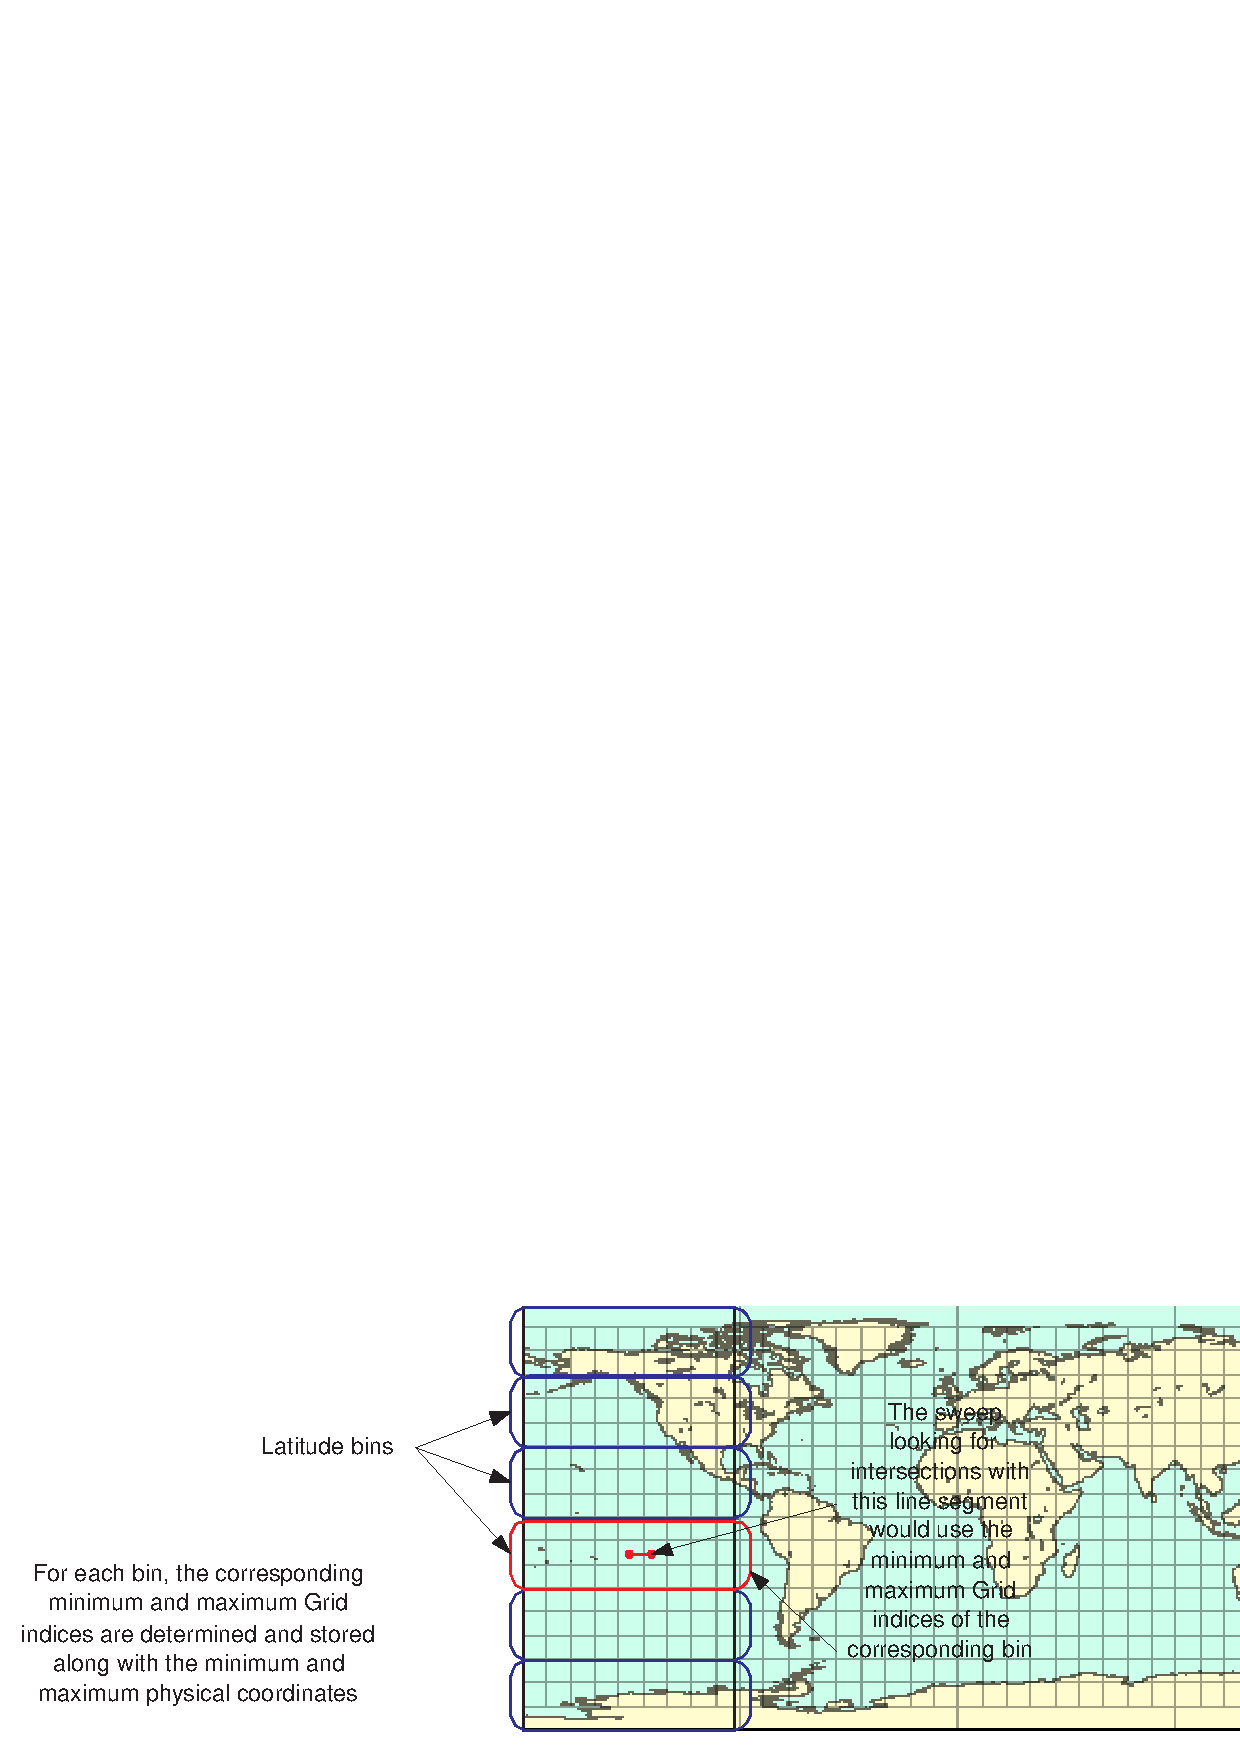
\includegraphics{ConservSweep2002}
\end{figure}
\end{center}

     Note that currently ESMF creates bins based
     only on coordinates in the second grid direction (typically "y" or "latitude").
     The second stage checks the bounding box of each grid cell in the determined
     bin.  The bounding box is formed by the cell's minimum and maximum coordinates.
     This process further restricts the actual sweep to a small number of cells.

     Once the sweep has been restricted, a robust algorithm that works for most
     cases is a cross-product test.  In this test, a cross product is computed
     between the vector corresponding to a cell side ($\vec{r}_{12}$ in
     Figure~\ref{fig:grids}) and a vector extending from the beginning of the
     cell side to the search point ($\vec{r}_{1b}$).  If 

\begin{equation}\label{eq:cross}
\vec{r}_{12} \times \vec{r}_{1b} > 0,
\end{equation}

     the point lies to the left of the cell side.  If (\ref{eq:cross}) holds for
     every cell side, the point is enclosed by the cell.  This test is not
     completely robust and will fail for grid cells that are non-convex.

% \subsubsection{Intersections}\label{sec:intersect}

     Once the location of an initial endpoint is found, it is necessary to check
     to see if the segment intersects with the cell side.  If the segment is
     parametrized as
\begin{eqnarray}
\theta &=& \theta_b + s_1 (\theta_e - \theta_b) \nonumber \\
\phi   &=& \phi_b + s_1 (\phi_e - \phi_b) 
\end{eqnarray}
     and the cell side as
\begin{eqnarray}
\theta &=& \theta_1 + s_2 (\theta_2 - \theta_1) \nonumber \\
\phi   &=& \phi_1 + s_2 (\phi_2 - \phi_1),
\end{eqnarray}
     where $\theta_1, \phi_1, \theta_2, \phi_2, \theta_b,$ and $\theta_e$ are
     endpoints as shown in Figure~\ref{fig:grids}, the intersection of the two
     lines occurs when $\theta$ and $\phi$ are equal.  The linear system 
\begin{equation}
\left[ \begin{array}{cc} 
(\theta_e - \theta_b) & (\theta_1 - \theta_2) \\
(\phi_e - \phi_b) & (\phi_1 - \phi_2) \\
\end{array} \right]
\left[ \begin{array}{c} s_1 \\ s_2 \\ \end{array} \right] = 
\left[ \begin{array}{c} 
(\theta_1 - \theta_b) \\ (\phi_1 - \phi_b)  \\
\end{array} \right]
\end{equation}
     is then solved to determine $s_1$ and $s_2$ at the intersection point.  If
     $s_1$ and $s_2$ are between zero and one, an intersection occurs with that
     cell side. 

     It is important also to compute identical intersections during the sweeps
     of each grid.  To ensure that this will occur, the entire line segment is
     used to compute intersections rather than using a previous or next
     intersection as an endpoint.

% \subsubsection{Coincidences}

     Often, pairs of grids will share common lines (e.g. the Equator).  When
     this is the case, the method described above will double-count the
     contribution of these line segments.  Coincidences can be detected when
     computing cross products for the search algorithm described above.  If
     the cross product is zero in this case, the endpoint lies on the cell
     side.  A second cross product between the line segment and the cell side
     can then be computed.  If the second cross product is also zero, the
     lines are coincident.  Once a coincidence has been detected, the
     contribution of the coincident segment can be computed during the
     first sweep and ignored during the second sweep.

% \subsubsection{Spherical coordinates}\label{sec-sphere}

     Some aspects of the spherical coordinate system introduce additional
     problems for the method described above.  Longitude is multiple valued
     on one line on the sphere, and this branch cut may be chosen differently
     by different grids.  Care must be taken when calculating intersections 
     and line integrals to ensure that the proper longitude values are used.
     A simple method is to always check to make sure the longitude is in the
     same interval as the source grid cell center.

     Another problem with computing weights in spherical coordinates is the
     treatment of the pole.  First, note that although the pole is physically
     a point, it is a line in latitude-longitude space and has a nonzero
     contribution to the weight integrals.  If a grid does not contain the
     pole explicitly as a grid vertex, the pole contribution must be added
     to the appropriate cells.  The pole contribution can be computed analytically.

     The pole also creates problems for the search and intersection algorithms
     described above.  For example, a grid cell that overlaps the pole can
     result in a nonconvex cell in latitude-longitude coordinates.  The
     cross-product test described above will fail in this case.  In addition,
     segments near the pole typically exhibit large changes in longitude even
     for very short segments.  In such a case, the linear parametrizations used
     above result in inaccuracies for determining the correct intersections.

     To avoid these problems, a coordinate transformation can be used poleward
     of a given threshold latitude (typically within one degree of the pole).
     A possible transformation is the Lambert equivalent azimuthal projection
\begin{eqnarray}
X &=& 2\sin\left({\pi \over 4} - {\theta \over 2}\right)\cos\phi \nonumber \\
Y &=& 2\sin\left({\pi \over 4} - {\theta \over 2}\right)\sin\phi 
\end{eqnarray}
     for the North Pole.  The transformation for the South Pole is similar.
     This transformation is only used to compute intersections; line integrals
     are still computed in latitude-longitude coordinates.  Because intersections
     computed in the transformed coordinates can be different from those computed
     in latitude-longitude coordinates, line segments which cross the latitude
     threshold must be treated carefully.  To compute the intersections
     consistently for such a segment, intersections with the threshold latitude
     are detected and used as a normal grid intersection to provide a clean break
     between the two coordinate systems.

%  \item [ESMF\_REGRID\_METHOD\_FILE]
%        Read a regrid from a file
%  \item [ESMF\_REGRID\_METHOD\_FOURIER]
%        Fourier transform.
%  \item [ESMF\_REGRID\_METHOD\_INDEX]
%        Index-space regrid (shift, stencil).
%  \item [ESMF\_REGRID\_METHOD\_LEGENDRE]
%        Legendre transform.
\item[ESMF\_REGRID\_METHOD\_LINEAR  ]
     This is a standard linear regridding algorithm for 1-d grids only.  In ESMF,
     it is used to regrid between vertical grids.

%  \item [ESMF\_REGRID\_METHOD\_NEARNBR]
%        Nearest-neighbor dist-weighted avg
\item [ESMF\_REGRID\_METHOD\_NONE]
     No regridding or undefined regrid.
%  \item [ESMF\_REGRID\_METHOD\_RASTER]
%        Regrid by rasterizing domain.
%  \item [ESMF\_REGRID\_METHOD\_REGRIDCOPY]
%        Copy existing regrid
%  \item [ESMF\_REGRID\_METHOD\_SHIFT]
%        Shift addresses of existing regrid
%  \item [ESMF\_REGRID\_METHOD\_SPLINE]
%        Cubic spline for 1-d regridding
%  \item [ESMF\_REGRID\_METHOD\_USER]
%        User-supplied method
\end{description}



\subsubsection{ESMF\_RegridNormOpt}

{\sf DESCRIPTION:\\}
Regrid normalization options supported by ESMF, for conservative regridding only.

Valid values are:
\begin{description}
   \item [ESMF\_REGRID\_NORM\_DSTAREA]
         The Regrid weights are normalized by the destination area of each cell. 
   \item [ESMF\_REGRID\_NORM\_FRACAREA]
         The Regrid weights are normalized by the area of the source grid
         overlapped by each cell (default).
   \item [ESMF\_REGRID\_NORM\_NONE]
         No normalization applied to Regrid weights.
   \item [ESMF\_REGRID\_NORM\_UNKNOWN]
         Unknown or undefined normalization.
\end{description}
